%% Editable source for result.pdf, written by make_result_figure.py from result.json
\documentclass[tikz,border=6pt]{standalone}
\usepackage[T1]{fontenc}
\begin{document}
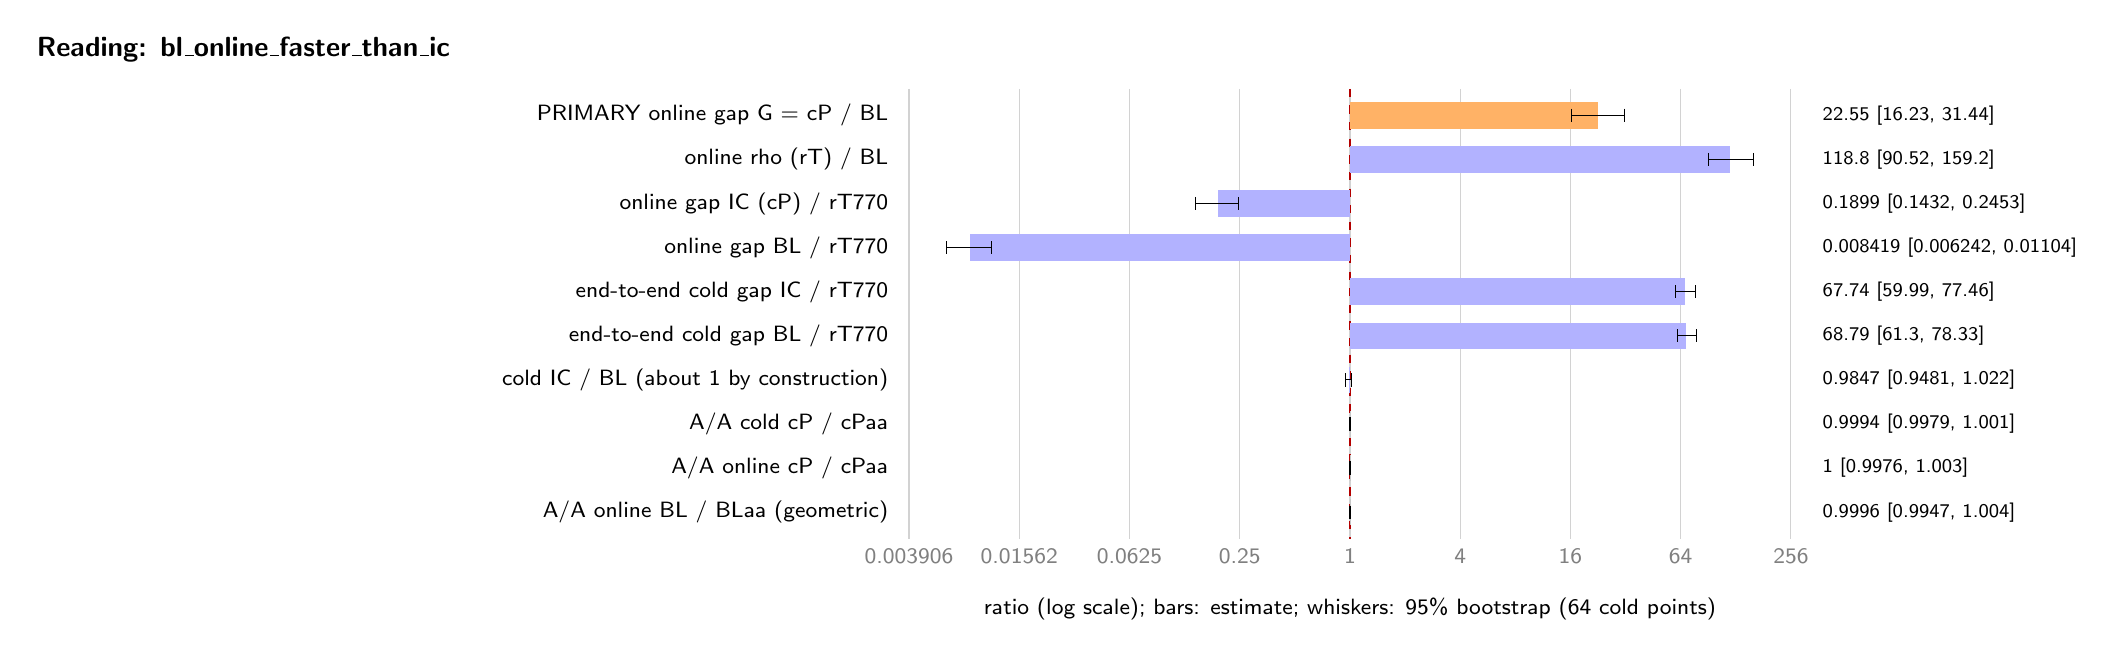
\begin{tikzpicture}[font=\sffamily\footnotesize,x=7mm,y=-5.6mm]
\draw[gray!35] (-8,-0.6) -- (-8,9.6); \node[gray] at (-8,10.0) {0.003906};
\draw[gray!35] (-6,-0.6) -- (-6,9.6); \node[gray] at (-6,10.0) {0.01562};
\draw[gray!35] (-4,-0.6) -- (-4,9.6); \node[gray] at (-4,10.0) {0.0625};
\draw[gray!35] (-2,-0.6) -- (-2,9.6); \node[gray] at (-2,10.0) {0.25};
\draw[gray!35] (0,-0.6) -- (0,9.6); \node[gray] at (0,10.0) {1};
\draw[gray!35] (2,-0.6) -- (2,9.6); \node[gray] at (2,10.0) {4};
\draw[gray!35] (4,-0.6) -- (4,9.6); \node[gray] at (4,10.0) {16};
\draw[gray!35] (6,-0.6) -- (6,9.6); \node[gray] at (6,10.0) {64};
\draw[gray!35] (8,-0.6) -- (8,9.6); \node[gray] at (8,10.0) {256};
\draw[red!70!black,dashed] (0,-0.6) -- (0,9.6);
\node at (0,11.2) {ratio (log scale); bars: estimate; whiskers: 95\% bootstrap (64 cold points)};
\node[anchor=west,font=\sffamily\bfseries] at (-24,-1.5) {Reading: bl\_online\_faster\_than\_ic};
\node[anchor=east] at (-8.2,0) {PRIMARY online gap G = cP / BL};
\fill[orange!60] (0,-0.30) rectangle (4.4953,0.30);
\draw (4.0209,0) -- (4.9747,0); \draw (4.0209,-0.15) -- (4.0209,0.15); \draw (4.9747,-0.15) -- (4.9747,0.15);
\node[anchor=west,font=\sffamily\scriptsize] at (8.4,0) {22.55 [16.23, 31.44]};
\node[anchor=east] at (-8.2,1) {online rho (rT) / BL};
\fill[blue!30] (0,0.70) rectangle (6.8921,1.30);
\draw (6.5002,1) -- (7.3148,1); \draw (6.5002,0.85) -- (6.5002,1.15); \draw (7.3148,0.85) -- (7.3148,1.15);
\node[anchor=west,font=\sffamily\scriptsize] at (8.4,1) {118.8 [90.52, 159.2]};
\node[anchor=east] at (-8.2,2) {online gap IC (cP) / rT770};
\fill[blue!30] (0,1.70) rectangle (-2.3968,2.30);
\draw (-2.8035,2) -- (-2.0275,2); \draw (-2.8035,1.85) -- (-2.8035,2.15); \draw (-2.0275,1.85) -- (-2.0275,2.15);
\node[anchor=west,font=\sffamily\scriptsize] at (8.4,2) {0.1899 [0.1432, 0.2453]};
\node[anchor=east] at (-8.2,3) {online gap BL / rT770};
\fill[blue!30] (0,2.70) rectangle (-6.8921,3.30);
\draw (-7.3238,3) -- (-6.5017,3); \draw (-7.3238,2.85) -- (-7.3238,3.15); \draw (-6.5017,2.85) -- (-6.5017,3.15);
\node[anchor=west,font=\sffamily\scriptsize] at (8.4,3) {0.008419 [0.006242, 0.01104]};
\node[anchor=east] at (-8.2,4) {end-to-end cold gap IC / rT770};
\fill[blue!30] (0,3.70) rectangle (6.0819,4.30);
\draw (5.9066,4) -- (6.2753,4); \draw (5.9066,3.85) -- (5.9066,4.15); \draw (6.2753,3.85) -- (6.2753,4.15);
\node[anchor=west,font=\sffamily\scriptsize] at (8.4,4) {67.74 [59.99, 77.46]};
\node[anchor=east] at (-8.2,5) {end-to-end cold gap BL / rT770};
\fill[blue!30] (0,4.70) rectangle (6.1041,5.30);
\draw (5.9377,5) -- (6.2916,5); \draw (5.9377,4.85) -- (5.9377,5.15); \draw (6.2916,4.85) -- (6.2916,5.15);
\node[anchor=west,font=\sffamily\scriptsize] at (8.4,5) {68.79 [61.3, 78.33]};
\node[anchor=east] at (-8.2,6) {cold IC / BL (about 1 by construction)};
\fill[blue!30] (0,5.70) rectangle (-0.0222,6.30);
\draw (-0.0769,6) -- (0.0307,6); \draw (-0.0769,5.85) -- (-0.0769,6.15); \draw (0.0307,5.85) -- (0.0307,6.15);
\node[anchor=west,font=\sffamily\scriptsize] at (8.4,6) {0.9847 [0.9481, 1.022]};
\node[anchor=east] at (-8.2,7) {A/A cold cP / cPaa};
\fill[gray!45] (0,6.70) rectangle (-0.0009,7.30);
\draw (-0.0031,7) -- (0.0012,7); \draw (-0.0031,6.85) -- (-0.0031,7.15); \draw (0.0012,6.85) -- (0.0012,7.15);
\node[anchor=west,font=\sffamily\scriptsize] at (8.4,7) {0.9994 [0.9979, 1.001]};
\node[anchor=east] at (-8.2,8) {A/A online cP / cPaa};
\fill[gray!45] (0,7.70) rectangle (0.0006,8.30);
\draw (-0.0035,8) -- (0.0045,8); \draw (-0.0035,7.85) -- (-0.0035,8.15); \draw (0.0045,7.85) -- (0.0045,8.15);
\node[anchor=west,font=\sffamily\scriptsize] at (8.4,8) {1 [0.9976, 1.003]};
\node[anchor=east] at (-8.2,9) {A/A online BL / BLaa (geometric)};
\fill[gray!45] (0,8.70) rectangle (-0.0006,9.30);
\draw (-0.0076,9) -- (0.0060,9); \draw (-0.0076,8.85) -- (-0.0076,9.15); \draw (0.0060,8.85) -- (0.0060,9.15);
\node[anchor=west,font=\sffamily\scriptsize] at (8.4,9) {0.9996 [0.9947, 1.004]};
\end{tikzpicture}
\end{document}
